\chapter{Assessing Damages Under Uncertainty}
\label{ch:damages}

\section{A number from a distribution}

Once liability is established, a court must put a number on the loss. The number is rarely known. A claimant injured at thirty will lose earnings over a working life whose length, wages and health are uncertain. A business whose contract was broken lost profits it might or might not have made. An investor misled into buying shares lost the difference between what she paid and what the shares would have been worth, a counterfactual price. In each case the court must turn a distribution of possible losses into a single award, usually a lump sum paid once and never revised. This chapter treats the assessment of damages as a Bayesian decision problem: form the posterior distribution of the loss, choose a loss function that reflects the law's objectives, and choose the award that minimises expected loss.\index{damages}

\section{The compensatory principle}

The basic principle in English and American law is that damages should put the claimant in the position she would have been in had the wrong not occurred, so far as money can. In contract, that is the position had the contract been performed; in tort, the position had the tort not been committed. Both are counterfactuals. Let $\theta$ be the claimant's loss, the difference in value between the counterfactual position and her actual position. The principle says the award should equal $\theta$. Since $\theta$ is uncertain, the court must estimate it.\index{compensatory principle}

\subsection{Which estimate?}

Decision theory says the right estimate depends on the loss function. If over compensation and under compensation by the same amount are equally bad, and badness grows with the square of the error, the optimal award is the posterior mean of $\theta$. If badness grows linearly, it is the posterior median. If under compensation is $k$ times as bad as over compensation, with linear loss, it is the posterior quantile at $k/(1+k)$. Each choice is defensible; the law rarely says which it is making.

The posterior mean has a special property: across many cases, awards equal to the mean compensate claimants as a class exactly on average, and defendants as a class pay, on average, the harm they caused. This aggregate accuracy matters for incentives, since defendants' expected liability then equals the expected harm, the condition for efficient care to which Chapter~\ref{ch:becker} returns, provided that every harm leads to a claim. For this reason we think the posterior mean is the default the law should adopt.

\section{Future losses}

\subsection{Lump sums and discounting}

Damages for future losses, such as lost earnings or the cost of care, are usually paid as a lump sum. The sum must be enough, invested, to provide the lost income over the relevant period. Two uncertain quantities determine it: the stream of future losses and the return on investment. English courts compute the lump sum using a multiplier\index{multiplier}, derived from actuarial tables known as the Ogden tables, applied to an annual loss, the multiplicand. The multiplier depends on the claimant's life expectancy or working life and on the discount rate, which is set by the Lord Chancellor under the Damages Act 1996. In \emph{Wells v Wells} the House of Lords held that the discount rate should reflect the return on index linked government stock, since claimants should not be required to take investment risk \citep{wells1999}. The rate has been changed several times since, including to a negative value in 2017, reflecting low real yields. The Civil Liability Act 2018 then departed from \emph{Wells}: the rate is now set on the assumption that the claimant invests in a low risk diversified portfolio, and on that basis it was set at minus one quarter of one per cent in 2019 and at plus one half of one per cent in 2025.\index{discount rate}\index{Ogden tables}

The discount rate matters a great deal. For a claimant with forty years of future loss, the multiplier for a fixed term of forty years, ignoring mortality, at a real rate of minus one quarter of one per cent is about forty two; at plus one half of one per cent it is about thirty six; at two and a half per cent it is about twenty five. A change in the rate of under three percentage points changes the award by more than a third. Setting the rate is a choice about who bears investment risk: a low rate protects claimants from poor returns, at a cost to defendants and their insurers.

\subsection{The predictive distribution}

A Bayesian assessment of future loss forms the predictive distribution of the present value of the loss, combining uncertainty about working life, wages and returns. Figure~\ref{fig:damages} shows a simulated example: a claimant with an expected remaining working life of twenty two years, with uncertainty, and an annual wage with uncertainty about its level, discounted at half of one per cent. The distribution is skewed: its mean exceeds its median, because high wages produce large losses. An award at the median would under compensate on average; an award at the mean would compensate the class exactly on average.

\begin{figure}[t]
\centering
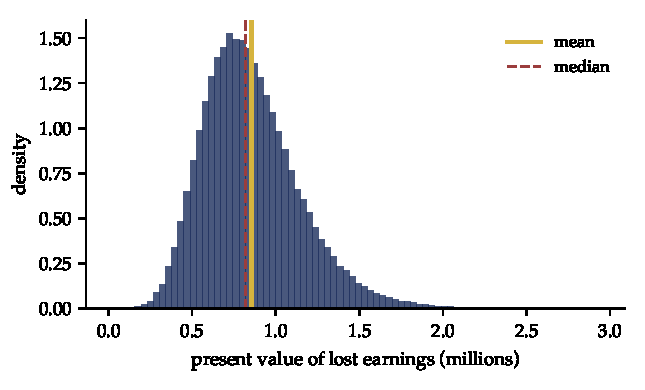
\includegraphics[width=\linewidth]{fig_damages}
\caption{Simulated predictive distribution of the present value of lost earnings, with uncertainty about working life and wages. The mean exceeds the median because the distribution is skewed to the right.}
\label{fig:damages}
\end{figure}

\subsection{Contingencies}

English courts adjust multipliers for contingencies other than mortality, such as unemployment, ill health and early retirement, using discounts in the Ogden tables that depend on the claimant's employment status, education and disability. These adjustments are expected value calculations: they reduce the award by the expected effect of events that would have reduced earnings in any case. Their basis is population data, and they can be individualised where the evidence supports it, by Bayesian updating of the population rates with evidence about the claimant.

\subsection{Periodical payments}

The Damages Act 1996, as amended by the Courts Act 2003, allows courts to order periodical payments\index{periodical payments} instead of a lump sum for future pecuniary loss, and requires them to consider whether such an order would be appropriate. Periodical payments, linked by default to the Retail Prices Index (earnings indexation, now usual for care costs, is available by a court order modifying the default, as in \emph{Thompstone v Tameside and Glossop Acute Services NHS Trust} \citep{thompstone2008}), transfer longevity and investment risk from the claimant to the defendant, who is usually an insurer or the National Health Service. In decision terms, they replace a point estimate of an uncertain quantity with a contract that pays the realised value. They remove the claimant's longevity risk, and they are used for the largest claims, such as those for catastrophic injury, where the uncertainty is greatest.

\section{Lost profits and the reasonable certainty rule}

\subsection{The rule}

American courts traditionally require that lost profits be proved with reasonable certainty, and have been reluctant to award profits for new businesses with no track record. In \emph{Story Parchment Co v Paterson Parchment Paper Co} the Supreme Court held in 1931 that where the fact of damage is certain, uncertainty about its amount does not bar recovery, and that the wrongdoer who created the uncertainty should bear its risk \citep{storyparchment1931}. English law follows similar principles: once loss is proved, the court must do its best to quantify it, and the difficulty of quantification is not a reason to award nothing.\index{lost profits}

\subsection{The Bayesian view}

The reasonable certainty rule conflates two questions. The first is whether there was a loss at all, a question of liability. The second is how large it was, a question of quantification. A Bayesian treats both as uncertain and integrates. If the probability that the business would have been profitable is $q$ and its expected profit if profitable is $\mu$, the expected loss is $q\mu$. A rule that awards nothing unless $q$ is high and awards $\mu$ if it is, is an all or nothing rule with the defects discussed in Chapter~\ref{ch:standards}. The proportional award $q\mu$ is the expected loss, and it gives the defendant the right incentives.

\subsection{Loss of a chance in contract}

English contract law has long accepted this logic. In \emph{Chaplin v Hicks} a theatre manager in breach of contract prevented the claimant from attending an interview in a beauty contest in which she was one of fifty finalists for twelve prizes; the Court of Appeal upheld an award for the loss of her chance, although it could not be known whether she would have won \citep{chaplin1911}. \emph{Allied Maples}, discussed in Chapter~\ref{ch:tort}, extended the principle to the hypothetical actions of third parties. Damages for a lost chance are the probability of success times the value of success, an expected value, discounted for any other contingencies.

\section{Damages against the wrongdoer}

\subsection{Evidential presumptions}

Where the defendant's wrong has made it impossible to measure the loss, courts often resolve uncertainty against the defendant. In \emph{Armory v Delamirie}, decided in 1722, a chimney sweep's boy found a jewel and took it to a goldsmith, whose apprentice removed the stones; the court directed the jury to presume the stones were of the finest water and assess damages accordingly, unless the goldsmith produced them \citep{armory1722}. The presumption is a rule about which posterior quantile to use: when the defendant has destroyed the evidence, the court uses a high quantile, shifting the cost of uncertainty to the party responsible for it.

In decision theoretic terms, the presumption serves an ex ante objective. If uncertainty were resolved at the posterior mean, a wrongdoer could profit from destroying evidence whenever the evidence would have shown a loss above the mean. Resolving uncertainty against the wrongdoer removes that incentive. The same logic underlies the adverse inference from a party's failure to call evidence it controls, and the rules on spoliation.

\subsection{Negotiating damages}

Where a defendant breaches a restrictive covenant over land or uses another's property without permission, courts may award damages measured by the sum the parties would reasonably have agreed for the release of the obligation. In \emph{Morris-Garner v One Step (Support) Ltd} the Supreme Court explained these negotiating damages\index{negotiating damages} as a measure of the value of the right lost, appropriate where that right was an asset with economic value \citep{morrisgarner2018}; the Court held that difficulty in proving financial loss is not by itself a reason to award them, and refused them on the facts, where the breach of non-compete covenants had caused ordinary financial loss. The hypothetical negotiation is a counterfactual bargaining problem: the court asks what two reasonable parties, with the information then available, would have agreed. A Bayesian treatment models each party's valuation and the bargaining outcome, such as the midpoint of the zone of agreement, using the information available at the date of the hypothetical negotiation.

\section{Hindsight in damages}

Should the assessment of damages use information that became available after the wrong? In \emph{Golden Strait Corporation v Nippon Yusen Kubishika Kaisha (The Golden Victory)} a charterer repudiated a charter with nearly four years to run, and the Second Gulf War, which would have entitled the charterer to cancel, broke out fifteen months later; the House of Lords held, by a majority, that damages should take account of the war, since the compensatory principle requires that the claimant receive no more than it would have received had the contract been performed \citep{goldenvictory2007}. The minority emphasised commercial certainty and the date of breach rule.

Chapter~\ref{ch:bankruptcy} returns to the same question in a different setting, the solvency of a firm judged after its failure. The Bayesian answer distinguishes the information set relevant to liability, which is fixed at the time of the act, from the information relevant to quantum, which can include later events because the loss itself unfolds over time. The posterior for the loss should condition on everything known at the date of assessment about events that would have affected the counterfactual position. \emph{The Golden Victory} is consistent with that principle; the minority's concern for certainty is a concern about the cost of uncertainty in commercial transactions, which is a legitimate input to the choice of rule.

\section{Experts and the combination of estimates}

Damages in commercial cases are often the subject of competing expert reports, using different models: discounted cash flows, comparable transactions, market prices. As Chapter~\ref{ch:fienberg} explains, experts are selected for favourable results, and the court sees two tails of the distribution of possible opinions. A Bayesian court treats each report as a signal, assesses its reliability, and combines them, rather than choosing one or splitting the difference. Where the experts agree on most inputs and disagree on a few, the court should focus on the disputed inputs and form its own posterior for each, then compute the damages implied. Judges do this informally when they accept one expert's discount rate and another's growth assumptions. Making the process explicit, with a table of inputs, the evidence for each and the resulting posterior, makes the judgment transparent and appealable on its merits.

\section{Interest and the time value of money}

A claimant compensated years after the loss has also lost the use of the money. Statutory and equitable interest compensate for this, at rates set by statute or by the court. The appropriate rate is a question about the claimant's counterfactual investment or borrowing, which is uncertain. In \emph{Sempra Metals v Inland Revenue Commissioners} the House of Lords allowed compound interest as restitutionary interest on tax paid under a mistake \citep{sempra2007}, though the Supreme Court has since held that no claim in unjust enrichment lies for compound interest on mistaken payments, so that this holding was overruled \citep{prudential2018}. Compound interest is the correct measure of the time value of money; simple interest systematically under compensates long delayed claims, a point of direct relevance to slow court systems such as those of Chapter~\ref{ch:india}.

\section{Damages in the age of data}

Data now inform damages more than ever. Earnings losses can be estimated from large panels of workers with similar characteristics; the costs of care from records of actual expenditure; the value of lost businesses from market data. Machine learning models can predict individual trajectories with uncertainty. These methods support the Bayesian approach of this chapter: they produce predictive distributions rather than point estimates, and they can be individualised by conditioning on the claimant's characteristics. The legal questions are which loss function to apply, whether to use the mean or another summary, and how to handle the risk that remains, by periodical payments, by insurance, or by accepting it.

\section*{Notes and Questions}
\addcontentsline{toc}{section}{Notes and Questions}
\begin{enumerate}[label=\arabic*.]
\item Compute the multiplier for forty years of annual loss at real discount rates of minus one quarter, plus one half and plus two and a half per cent. By what percentage does the award fall between the first and last?
\item A claimant's working life is uncertain, with mean twenty years and standard deviation five. Show by simulation that the expected present value is less than the present value at the expected working life when the discount rate is positive, and greater when it is negative. Why?
\item A start up's chance of becoming profitable was forty per cent, and its expected profits if profitable were five million. Under the reasonable certainty rule, what would a court likely award? Under the expected value approach?
\item In \emph{Chaplin v Hicks}, the claimant was one of fifty finalists for twelve prizes. What was her chance of a prize? How should the court value it?
\item Explain the presumption in \emph{Armory v Delamirie} as a choice of posterior quantile. What incentive does it create?
\item Should \emph{The Golden Victory} be followed in a market where contracts are routinely traded? Frame your answer in terms of the cost of uncertainty.
\end{enumerate}

\section*{Further reading}
\emph{Wells v Wells} on discounting \citep{wells1999}; \emph{Story Parchment} on uncertain damages \citep{storyparchment1931}; \emph{Morris-Garner} on negotiating damages \citep{morrisgarner2018}; \emph{The Golden Victory} on hindsight \citep{goldenvictory2007}; \emph{Chaplin v Hicks} on loss of a chance \citep{chaplin1911}; \emph{Armory v Delamirie} on evidential presumptions \citep{armory1722}; \emph{Sempra Metals} on interest \citep{sempra2007}.
